\chapter{Boundary Conditions}

\section{Heat Flux}
Given a boundary segment we can prescribe the a heat flux normal to that boundary as
\begin{equation}
	\lambda \left(\vec{n} \cdot \nabla T \right) = \dot{q}_{\perp}
\end{equation}
where $\lambda$ is the thermal conductivity, $\vec{n}$ the normal vector of the boundary, $\nabla T$ the temperature gradient at a given point in the cell and $\dot{q}_{\perp}$ the differential heat flux perpendicular to the boundary.

We use linear element as our ansatz function for $T$ and triangles as cells which means that $\vec{n}$ and $\nabla T$ are constants.
If we now assume a per cell constant thermal conductivity $\lambda$ this means that the differential heat flux $\dot{q}_{\perp}$ must be constant over a given cell side.

Using the FEM ansatz with linear tetrahedral elements we can write
\begin{equation}
	\lambda \int_0^1 \int_0^{1 - \eta} \left( \vec{n} \cdot \nabla T \right) \phi_0 \det\left( \mm{J}(x, y) \right) \diff{\xi} \diff{\eta} = \dot{q}_{\perp} \int_0^1 \int_0^{1 - \eta} \phi_0 \det\left( \mm{J}(x, y) \right) \diff{\xi} \diff{\eta}.
\end{equation}
Assuming the boundary is the button one the normal vector is simply
\begin{equation}
	\vec{n} = 
	\begin{pmatrix}
	0\\
	-1
	\end{pmatrix}
\end{equation}
which leads to
\begin{equation}
	\vec{n} \cdot \nabla T = -\pdv{T}{y} = \frac{T_0(\Delta x_1 - \Delta x_2) + T_1 \Delta x_2 - T_2 \Delta x_1}{\det\left(\mm{J}(x,y)\right)}
\end{equation}
which leads to
\begin{align}
	\left( T_0(\Delta x_1 - \Delta x_2) + T_1 \Delta x_2 - T_2 \Delta x_1\right) &\iint \phi_0 \diff{\xi} \diff{\eta} =\\
	\frac{\dot{q} \det\left( \mm{J}(x, y) \right)}{\lambda} &\iint \phi_0 \diff{\xi} \diff{\eta}
\end{align}
\begin{equation}
	\boxed{T_0(\Delta x_1 - \Delta x_2) + T_1 \Delta x_2 - T_2 \Delta x_1 =
	\frac{\dot{q}}{\lambda} \det\left( \mm{J}(x, y) \right).}
\end{equation}
Assuming the boundary is on the left we get to a similar argumentation to
\begin{equation}
	\boxed{T_0(\Delta y_2 - \Delta y_1) - T_1\Delta y_2 + T_2\Delta y_1 =
	\frac{\dot{q}}{\lambda} \det\left( \mm{J}(x, y) \right)}.
\end{equation}

\section{Radiation}
The net radiation heat flux from surface 1 to surface 2 using grey body radiation can be calculated as 
\begin{equation}
	\dot{Q}_{1 \rightarrow 2} = A_1 F_{1 \rightarrow 2} E_1 -  A_2 F_{2 \rightarrow 1} E_2.
\end{equation}
using the formula for emission of grey bodies
\begin{equation}
	E_i = \epsilon_i \sigma T_i^4 
\end{equation}
and the reciprocity rule for configuration factors $A_1 F_{1 \rightarrow 2} = A_2 F_{2 \rightarrow 1}$ we can write
\begin{equation}
	\dot{Q}_{1 \rightarrow 2} = \sigma A_1 F_{1 \rightarrow 2} \left(\epsilon_1 T1^4 - \epsilon_2 T_2^4\right)
\end{equation}
and $\dot{Q}_{1 \rightarrow 2} = -\dot{Q}_{2 \rightarrow 1}$.
Given two line segments as seen in Fig.~\ref{fig:radiation}
%---------------------------------------------------------------------------------------------------------------
\begin{figure}[H]
	\centering
	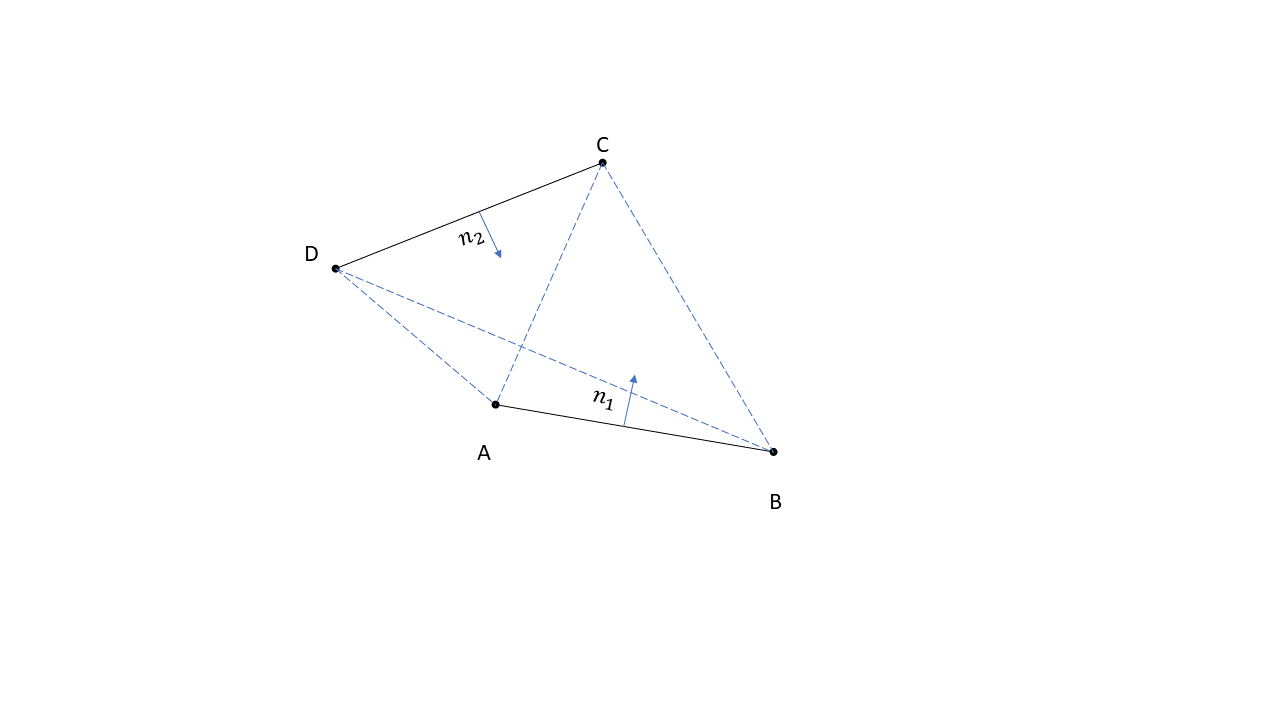
\includegraphics[trim= 8cm 5cm 13cm 3.5cm ,clip,width=0.6\textwidth]{figures/radiation.png}
	\caption{Radiation.}
	\label{fig:radiation}
\end{figure}
%---------------------------------------------------------------------------------------------------------------
the configuration factor from surface $\overline{\mm{AB}}$ to surface $\overline{\mm{CD}}$ can be calculated as
\begin{equation}
	F_{\overline{\mm{AB}} \rightarrow \overline{\mm{CD}}} = \frac{\overline{\mm{AC}} + \overline{\mm{BD}} - \overline{\mm{AD}} - \overline{\mm{BC}}}{2 \overline{\mm{AB}}}
\end{equation}
where $\overline{\mm{XY}}$ is the distance from $\mm{X}$ to $\mm{Y}$.
The total heat flux from or to a single surface is the sum of the heat fluxes to other surfaces plus the heat flux to the background
\begin{align}
	\dot{Q}_{tot} = \sigma A_1 \left\{\epsilon_1 T_1^4 \sum_i F_{1 \rightarrow i} - \sum_i \epsilon_i F_{1 \rightarrow i}  T_i^4 \right\} + \dot{Q}_{backgr}\\
	\dot{Q}_{tot} = \sigma A_1 \left\{\epsilon_1 T_1^4 \sum_i F_{1 \rightarrow i} - \sum_i \epsilon_i F_{1 \rightarrow i}  T_i^4  +  F_{1 \rightarrow bg} (\epsilon_i T_1^4 - \epsilon_{bg} T_{bg}^4) \right\}
\end{align}
Since $F_{1 \rightarrow bg} = 1 - \sum_i F_{1 \rightarrow i} $ we get
\begin{equation}
	\dot{Q}_{tot} = \sigma A_1 \left\{\epsilon_1 T_1^4  - \sum_i \epsilon_i F_{1 \rightarrow i}  T_i^4  - F_{1 \rightarrow bg} ) \epsilon_{bg} T_{bg}^4 \right\}
\end{equation}

In terms of boundary conditions, using $\dot{q}_{1 \rightarrow 2} = \dot{Q}_{1 \rightarrow 2} / A_1$,we ca write
\begin{equation}
	\lambda \left(\vec{n} \cdot \nabla T \right) = \dot{q}_{1 \rightarrow 2}
\end{equation}